\chapter{Background}
\label{chap:background}

In this chapter, we provide the relevant technical background required to understand our work. We start by introducing the optimisation problem in \cref{sec:optimisation_problem}. This is continued by a mathematical formulation of the optimisation landscape in \cref{sec:optimisation_landscape}. We then discuss optimisation in deep learning in \cref{sec:optimisation_in_deep_learning}. We end this chapter with a discussion of computationally tractable methods for curvature exploitation in \cref{sec:tractable_curvature_exploitation}.

\section{The Optimisation Problem}
\label{sec:optimisation_problem}

In this section, we formalise the optimisation problem. In the most fundamental case, we minimise an objective function $f$ with respect to real-valued variables with no constraints. The formulation is 
\begin{align}
    \min_{x} f(x)
\end{align}
where
\begin{itemize}
    \item $x \in \mathbb{R}^n$ is a real-valued vector with $n \geq 1$ components,
    \item $f: \mathbb{R}^n \to \mathbb{R}$ is a real-valued function,
    \item $f \in C^k$ s.t. $k \geq 1$ is smooth.
\end{itemize}
We only have a local perspective of $f$, since it is usually expensive to evaluate. We only know what $f$ evaluates to on a limited set of points $x_0, x_1, \ldots, x_k$, in which we use this information to find an optimal point $x^*$ that minimises $f$, as the solution. To do this, we must understand the landscape of $f$ and the scenarios that arise when traversing it.

\section{The Optimisation Landscape}
\label{sec:optimisation_landscape}
In this section, we introduce fundamental concepts that describe the landscape of $f$, which are needed to develop and analyse optimisation algorithms. Here, we introduce the notion of critical points, convexity, and ill-conditioning.

\subsection{Critical Points}
\label{ssec:critical_points}

When exploring the landscape of an objective function, we are interested in identifying specific points of interest that characterise its features. These are called \textit{critical points}. The most desirable of these are \textit{global optima}, in which there are \textit{global minimum} or \textit{global maximum}. An example is provided in \cref{fig:global_min_max}.

\begin{definition}[Global Minimum]
    A point $x^*$ is a \textit{global minimum} if $f(x^*) \leq f(x)$ for all $x$ in the entire domain of $f$.
\end{definition}

\begin{definition}[Global Maximum]
    A point $x^*$ is a \textit{global maximum} if $f(x^*) \geq f(x)$ for all $x$ in the entire domain of $f$.
\end{definition}

\begin{figure}[h]
    \begin{subfigure}[b]{0.48\linewidth}
        \centering
        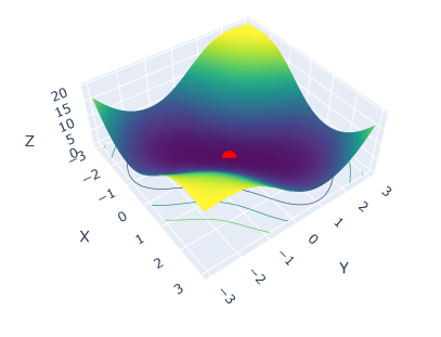
\includegraphics[width=\linewidth]{figures/2background/glob_min.png}
        \caption{A global minimum on $f(x,y) = x^2 + y^2$.}
        \label{fig:global_min}
    \end{subfigure}
    \hfill
    \begin{subfigure}[b]{0.48\linewidth}
        \centering
        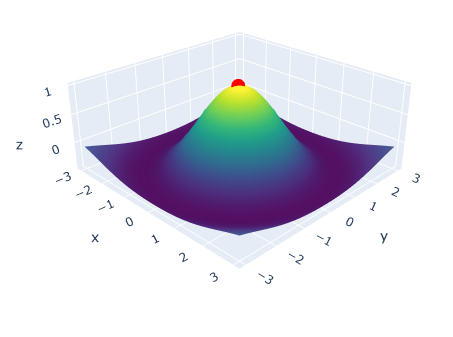
\includegraphics[width=\linewidth]{figures/2background/glob_max.png}
        \caption{A global maximum on \\
        $f(x,y) = \cos(x^2 + y^2) e^{-0.1 (x^2 + y^2)}$.}
        \label{fig:global_max}
    \end{subfigure}
    \caption{Examples of global minimum and maximum marked in red.}
    \label{fig:global_min_max}
\end{figure}

Finding such global optima is challenging, as we only have a limited set of information about $f$ and are resource constrained. Thus, many optimisation algorithms aim to find \textit{local optima}, which are points that are locally optimal. Similarly, there are \textit{local minimum} or \textit{local maximum}. We define these points with respect to a neighbourhood $\mathcal{N}$ of a point $x$. We provide examples in \cref{fig:local_min_max}.

\begin{definition}[Local Minimum]
    A point $x^*$ is a \textit{local minimum} if there exists a neighbourhood $\mathcal{N}$ around $x^*$ such that $f(x^*) \leq f(x)$ for all $x \in \mathcal{N}$. It is a \textit{strict local minimum} if instead $f(x^*) < f(x)$ for all $x \in \mathcal{N} \setminus \{x^*\}$.
\end{definition}

\begin{definition}[Local Maximum]
    A point $x^*$ is a \textit{local maximum} if there exists a neighbourhood $\mathcal{N}$ around $x^*$ such that $f(x^*) \geq f(x)$ for all $x \in \mathcal{N}$. It is a \textit{strict local maximum} if instead $f(x^*) > f(x)$ for all $x \in \mathcal{N} \setminus \{x^*\}$.
\end{definition}

\begin{figure}[h]
    \begin{subfigure}[b]{0.48\linewidth}
        \centering
        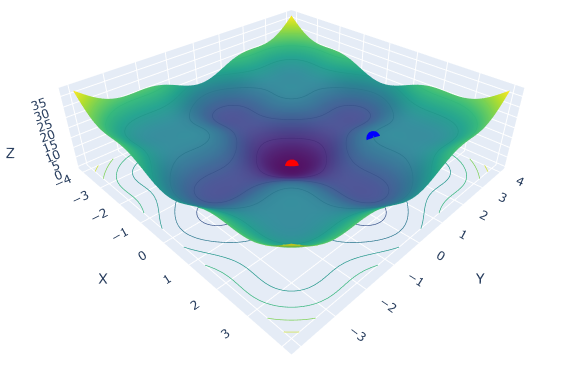
\includegraphics[width=\linewidth]{figures/2background/local_min.png}
        \caption{A local minimum on the egg crate function. \\
        $f(x,y) = (x^2 + y^2) + 5 * (\sin(x)^2 + \sin(y)^2)$.
        }
        \label{fig:local_min}
    \end{subfigure}
    \hfill
    \begin{subfigure}[b]{0.48\linewidth}
        \centering
        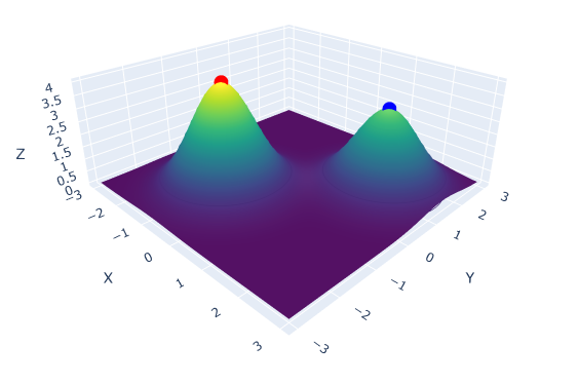
\includegraphics[width=\linewidth]{figures/2background/local_max.png}
        \caption{A local maximum on a multi-bump function. \\
        $f(x,y) = 3 e^{-(x-1.5)^2 - (y-1.5)^2} + \\
         4 e^{-(x+1)^2 - (y+1)^2}$.}
        \label{fig:local_max}
    \end{subfigure}
    \caption{Examples of local minimum and maximum marked in blue. The global minimum and maximum are marked in red for comparison.}
    \label{fig:local_min_max}
\end{figure}

Beyond these, we have \textit{saddle points}. These are points that are locally flat but are neither a local minimum nor a local maximum, as seen in \cref{fig:saddle_point}. In any neighbourhood $\mathcal{N}$ around a saddle point, the function's value increases along some directions emanating from $x^*$ and decreases along others.

\begin{figure}[h]
    \begin{subfigure}[b]{0.48\linewidth}
        \centering
        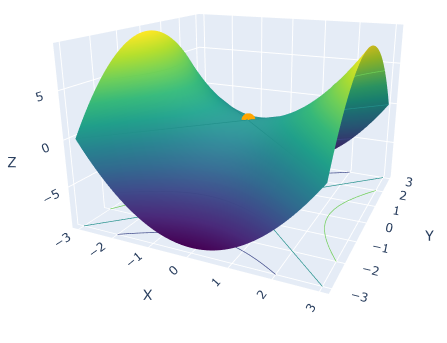
\includegraphics[width=0.8\linewidth]{figures/2background/horse_saddle.png}
        \caption{A saddle point on the horse saddle function. \\
        $f(x,y) = x^2 - y^2$.}
        \label{fig:horse_saddle}
    \end{subfigure}
    \hfill
    \begin{subfigure}[b]{0.48\linewidth}
        \centering
        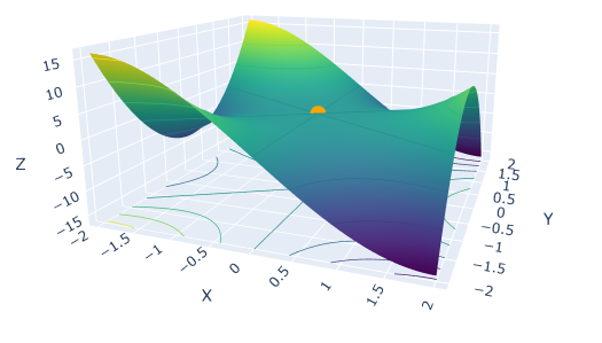
\includegraphics[width=\linewidth]{figures/2background/monkey_saddle.png}
        \caption{A saddle point on the monkey saddle function. \\
        $f(x,y) = x^3 - 3xy^2$.}
        \label{fig:monkey_saddle}
    \end{subfigure}
    \caption{Examples of functions containing saddle points marked in orange.}
    \label{fig:saddle_point}
\end{figure}

\subsection{Recognising Critical Points}
\label{ssec:recognising_critical_points}

For smooth and differentiable functions, we can recognise critical points using the first and second order information about $f$. Here, we introduce the necessary conditions that we can use to recognise them. We restrict our attention to the class of functions where $f \in C^k$ for $k \geq 2$.

A key property of any critical point $x^*$ is that $f$ is locally flat at $x^*$. This implies that its gradient---the vector of \textit{first-order} partial derivatives, $\nabla f(x^*)$---must be zero. These are called \textit{stationary points}.
\begin{definition}[Stationary Point]
    A point $x^*$ is a \textit{stationary point} if its gradient is zero:
    \begin{align}
        \nabla f(x^*) = 0.
    \end{align}
\end{definition}

We note that all stationary points are critical points, but not all critical points are stationary points. For example, a function may have a critical point at a point where the gradient is undefined. However, as mentioned, given we restrict our attention to twice-differentiable functions, we do not need to consider this case. 

All global optima, local optima and saddle points are stationary points, but not all stationary points are optima. To distinguish between them, we examine the function's \textit{local curvature} at $x^*$, which is captured by the \textit{Hessian matrix}---an $n \times n$ symmetric matrix of \textit{second-order} partial derivatives of $f$, denoted $\nabla^2 f(x)$ for a point $x$. We abbreviate the Hessian matrix for a function $f$ at a point $x$ as $H$ for convenience. The curvature information captured by $H$ can be summarised by its \textit{eigenvalues}. We denote a particular eigenvalue of $H$, and more generally any matrix, as $\lambda_i$. We use these eigenvalues of $H$ at a stationary point $x^*$ to allow for its classification.

\begin{itemize}
    \item If $H$ is \textit{positive semi-definite}, where all eigenvalues $\lambda_i \geq 0$ for all $i \in [1, n]$, then $x^*$ is a local minimum. 
    \item If $H$ is \textit{negative semi-definite}, where all eigenvalues $\lambda_i \leq 0$ for all $i \in [1, n]$, then $x^*$ is a local maximum.
\end{itemize}

\textbf{TODO: Diagram of Hessian matrix and its eigenvalues (? - not sure if this is needed)}

A special case is when $H$ is \textit{indefinite}, where eigenvalues $\lambda_i$ are not all positive or negative, and are a mixture of both. In this case, the function curves upwards in some directions and downwards in others. This is a saddle point.

\begin{definition}[Saddle Point]
    A point $x^*$ is a \textit{saddle point} if $H$ is indefinite.
\end{definition}

Now, we can classify between local minima, local maxima, and saddle points using the Hessian matrix. However, we can guarantee something stronger, and can distinguish between local minima/maxima and strict local minima/maxima.

\begin{itemize}
    \item If $H$ is \textit{positive definite}, where all eigenvalues $\lambda_i > 0$ for all $i \in [1, n]$, then $x^*$ is a strict local minimum. This signifies that the function curves upwards in all directions from $x^*$.
    \item If $H$ is \textit{negative definite}, where all eigenvalues $\lambda_i < 0$ for all $i \in [1, n]$, then $x^*$ is a strict local maximum. This signifies that the function curves downwards in all directions from $x^*$.
\end{itemize}

This is a stronger condition than positive/negative semi-definiteness, and is a sufficient condition for recognising a local minimum/maximum. If the Hessian at a stationary point is merely positive semidefinite, $x^*$ could be a local minimum or a flat region that is not a strict minimum. Similarly, if $H(x^*)$ is negative semidefinite, $x^*$ could be a local maximum or a flat region. With this we can guarantee a direction of movement from $x^*$ that will optimise $f$, without getting stuck in a flat region. 

\subsection{Convexity and Global Optimality}
\label{ssec:convexity}

The property of convexity significantly simplifies the task of characterising and finding optimal solutions. A function $f: \mathbb{R}^n \to \mathbb{R}$ is termed \textit{convex} if its domain is a convex set and for any two points $x_1, x_2$ in its domain, and any scalar $\lambda \in [0, 1]$:
\begin{align}
    f(\lambda x_1 + (1-\lambda)x_2) \leq \lambda f(x_1) + (1-\lambda)f(x_2)
    \label{eq:convexity_definition}
\end{align}
Geometrically, this implies that the line segment connecting any two points on the function's graph lies on or above the graph itself. For a twice-differentiable function, convexity is equivalent to its Hessian matrix $H(x)$ being positive semidefinite for all $x$ in its domain.

Convex functions are particularly appealing in optimisation due to two key properties:
\begin{itemize}
    \item Any local minimum of a convex function is also a global minimum. This means that if an algorithm finds a local minimum, it has successfully found the best possible solution.
    \item If a convex function is also differentiable, then any stationary point (where $\nabla f(x^*) = 0$) is guaranteed to be a global minimum.
\end{itemize}
These properties remove the concern of optimisation algorithms getting trapped in local minima that are not globally optimal, a common challenge in non-convex optimisation, which will be discussed later.

\subsection{Ill-Conditioning}


\section{Optimisation in Deep Learning}
\label{sec:optimisation_in_deep_learning}

% The optimisation principles discussed earlier are key, but applying them in deep learning brings unique challenges. Deep neural networks have vast parameter spaces and very complex, non-convex loss landscapes. This section examines these specific challenges and introduces the main classes of algorithms used to navigate them.

% \subsection{Challenges in High-Dimensional Landscapes}
% \label{ssec:dl_challenges}

% The "curse of dimensionality" is especially evident in deep learning. Models can have millions or even billions of parameters, creating very complex loss landscapes. A key result is the increase in \textit{saddle points} rather than poor local minima. Important studies by \citet{dauphin2014sfn} and \citet{choromanska2015loss} showed that for the high-dimensional, non-convex functions common in neural networks, saddle points become exponentially more frequent than local minima as dimension increases. Additionally, many local minima found in deep learning often have loss values close to the global minimum, making saddle points a greater obstacle to training.

% Saddle points are a major challenge for optimisation algorithms:
% \begin{itemize}
%     \item \textbf{First-order methods}, using only gradient information, can slow down greatly or get stuck near saddle points. The gradient magnitude can be very small near a saddle point, making these methods see the region as flat and progress very little. They don't have curvature information to find escape routes.
%     \item \textbf{Classical second-order methods}, like Newton's method, also face difficulties. If the Hessian at a saddle point has negative eigenvalues (showing negative curvature), the Newton step might move away from the saddle (possibly to areas of higher loss if not handled carefully) or even towards it if the gradient aligns with positive curvature directions.
% \end{itemize}
% Successfully handling these saddle points, not just avoiding bad local minima, is therefore key in deep learning optimisation.

% \subsection{First-Order Methods}
% \label{ssec:first_order_methods}

% First-order optimisation methods are widely used in deep learning because they are computationally efficient and scalable. These methods use the first derivative (gradient) of the objective function to find a minimum.

% \subsubsection{Gradient Descent (GD)}
% The simplest first-order algorithm is Gradient Descent (GD). It repeatedly updates parameters $\theta$ against the gradient of the objective function $f(\theta)$:
% \begin{align}
%     \theta_{t+1} = \theta_t - \alpha \nabla f(\theta_t)
%     \label{eq:gd_update}
% \end{align}
% where $\alpha > 0$ is the \textit{learning rate}, a scalar controlling the step size. While simple, computing the full gradient $\nabla f(\theta_t)$ means evaluating the function over the entire training dataset, which is too computationally expensive for the large datasets often used in deep learning.

% \subsubsection{Stochastic Gradient Descent (SGD)}
% To handle GD's computational cost, Stochastic Gradient Descent (SGD) is commonly used. Instead of the full dataset, SGD estimates the gradient using a small, random data sample called a \textit{mini-batch}. If $g_t(\theta_t)$ is this stochastic gradient estimate at iteration $t$, the update is:
% \begin{align}
%     \theta_{t+1} = \theta_t - \alpha g_t(\theta_t)
%     \label{eq:sgd_update}
% \end{align}
% This greatly reduces the cost per iteration. The randomness adds noise to the gradient estimates, which can help the optimiser escape sharp local minima. But this noise can also slow convergence because updates aren't always in the true steepest descent direction. Mini-batch SGD (often just called SGD in deep learning) is standard practice.

% \subsubsection{Momentum}
% To speed up SGD and reduce oscillations from noisy gradients, \textit{momentum} is often used. Inspired by physics, momentum methods build up an average of past gradients and keep moving in that direction. A common update is:
% \begin{align}
%     v_{t+1} &= \beta v_t + (1-\beta) g_t(\theta_t) \label{eq:momentum_velocity} \\
%     \theta_{t+1} &= \theta_t - \alpha v_{t+1} \label{eq:momentum_update}
% \end{align}
% where $v_t$ is the momentum (or velocity) at iteration $t$, and $\beta \in [0,1)$ is the momentum coefficient. Often, $(1-\beta)$ is part of the learning rate for $g_t$, or a different formula like $v_{t+1} = \beta v_t + \alpha g_t(\theta_t)$ is used, followed by $\theta_{t+1} = \theta_t - v_{t+1}$. The main idea is that updates gain momentum in consistent gradient directions and reduce variations from different mini-batches.

% \subsection{Second-Order Methods}
% \label{ssec:second_order_methods}

% Second-order optimisation methods use curvature information from the objective function, usually with the Hessian matrix. This provides a more direct route to the minimum, especially for poorly shaped landscapes.

% \subsubsection{Newton's Method}
% Newton's method forms a second-order Taylor expansion (a quadratic model) of $f$ around the current point $\theta_t$:
% \begin{align}
%     f(\theta_t + p) \approx f(\theta_t) + \nabla f(\theta_t)^T p + \frac{1}{2} p^T H(\theta_t) p
% \end{align}
% where $H(\theta_t) = \nabla^2 f(\theta_t)$ is the Hessian. The next step $p_t$ comes from minimizing this quadratic model, giving the Newton step:
% \begin{align}
%     p_t = -[H(\theta_t)]^{-1} \nabla f(\theta_t)
%     \label{eq:newton_step}
% \end{align}
% Parameters are updated: $\theta_{t+1} = \theta_t + p_t$. Newton's method can converge quickly (quadratically) near a minimum if the Hessian is positive definite. However, it has major drawbacks for deep learning:
% \begin{itemize}
%     \item \textbf{Computational Cost}: Storing the Hessian takes $O(N^2)$ memory, and inverting it takes $O(N^3)$ operations for $N$ parameters. This is not practical for typical neural networks.
%     \item \textbf{Non-Positive Definite Hessian}: If $H(\theta_t)$ is not positive definite (like near saddle points or areas of negative curvature), the Newton step might not reduce the objective value and could even increase it.
% \end{itemize}

% \subsubsection{Saddle-Free Newton (SFN) Method}
% To fix Newton's method's problems with non-positive definite Hessians, especially how it handles saddle points, changes like the Saddle-Free Newton (SFN) approach exist. The main idea is to change the Hessian matrix $H_t$ so the search direction always reduces the objective and can escape saddles. This is often done by changing its eigenvalues, for instance, by taking their absolute values:
% \begin{align}
%     H_t^{SFN} = V |\Lambda| V^T
%     \label{eq:sfn_hessian}
% \end{align}
% where $H_t = V \Lambda V^T$ is the eigendecomposition of the Hessian, and $|\Lambda|$ is a diagonal matrix with the absolute values of the eigenvalues. The update is then:
% \begin{align}
%     p_t = -[H_t^{SFN}]^{-1} \nabla f(\theta_t)
%     \label{eq:sfn_step}
% \end{align}
% This helps the optimiser treat saddle points like minima from the viewpoint of the changed Hessian, making it easier to escape them. Although SFN solves the saddle point issue for Newton-like methods, it still has the high computational costs of creating, decomposing, and inverting an $N \times N$ Hessian matrix if computed directly.

\section{Methods for Tractable Curvature Exploitation}
\label{sec:tractable_curvature_exploitation}

% While second-order methods like Newton's method offer the promise of rapid convergence by leveraging curvature information, their direct application in deep learning is often crippled by the prohibitive computational cost of forming, storing, and inverting the Hessian matrix. This section introduces techniques that aim to harness curvature information in a more computationally feasible manner.

% \subsection{Krylov Subspace Methods}
% \label{ssec:krylov_methods}

% Krylov subspace methods provide a powerful framework for approximating the solutions to large linear systems or eigenvalue problems without explicitly forming the matrices involved. In the context of optimisation, particularly for approximating the Newton step $p_t = -[H(\theta_t)]^{-1} \nabla f(\theta_t)$, these methods allow us to work with a much smaller, carefully chosen subspace of the full parameter space.

% Given an $N \times N$ matrix $A$ (in our case, often the Hessian $H$) and a vector $v$ (often the gradient $g = \nabla f(\theta_t)$ or the negative gradient), the $m$-th Krylov subspace, denoted $\mathcal{K}_m(A, v)$, is defined as the span of the vectors $\{v, Av, A^2v, \ldots, A^{m-1}v\}$:
% \begin{align}
%     \mathcal{K}_m(A, v) = \text{span}\{v, Av, A^2v, \ldots, A^{m-1}v\}
%     \label{eq:krylov_subspace_definition}
% \end{align}
% Typically, $m \ll N$. The intuition is that this subspace contains rich information about the action of $A$ on $v$. Instead of solving the full $N$-dimensional Newton system $H p = -g$, one can seek an approximate solution $p_m$ that lies within this $m$-dimensional Krylov subspace. This effectively reduces the problem to solving a much smaller system.

% The key to the computational efficiency of Krylov subspace methods is that the basis vectors $v, Av, \ldots, A^{m-1}v$ can be generated iteratively through repeated \textit{matrix-vector products} (in our context, Hessian-vector products, or HvPs, of the form $Hw$ for some vector $w$). Crucially, these HvPs can often be computed efficiently without explicitly forming the full Hessian matrix $H$. Techniques such as automatic differentiation (as used in backpropagation) can be extended to calculate HvPs at a cost that is only a small constant factor more than computing the gradient itself.

% By restricting the search for a direction to a low-dimensional Krylov subspace, these methods can capture dominant curvature information and produce effective Newton-like steps or approximations thereof, while avoiding the $O(N^2)$ storage and $O(N^3)$ computation associated with the explicit Hessian. Algorithms like the Conjugate Gradient (CG) method, a prominent Krylov subspace method, iteratively build up such a subspace to solve linear systems like the Newton equations.
